\subsection{Backend}

\begin{frame}[fragile]{Backend}
	\begin{figure}
	  \begin{center}
	    \leavevmode
	      \includegraphics[width = .75\textwidth]{backend}
	    \caption{Team Backend}
	  \end{center}
	\end{figure}
\end{frame}

\begin{frame}[fragile]{JVM Bytecode und Classfile}
% NB. listings is quite powerful, but not well suited to be used with beamer
%  consider using semiverbatim or the like, see below
\begin{lstlisting}[language=Java]
public class HelloWorld{
	  public static void main(String[] args){
	    System.out.println("Hello World");
	  }	
}
\end{lstlisting}
\end{frame}

\begin{frame}[fragile]{Classfile Beispiel}
\begin{center}
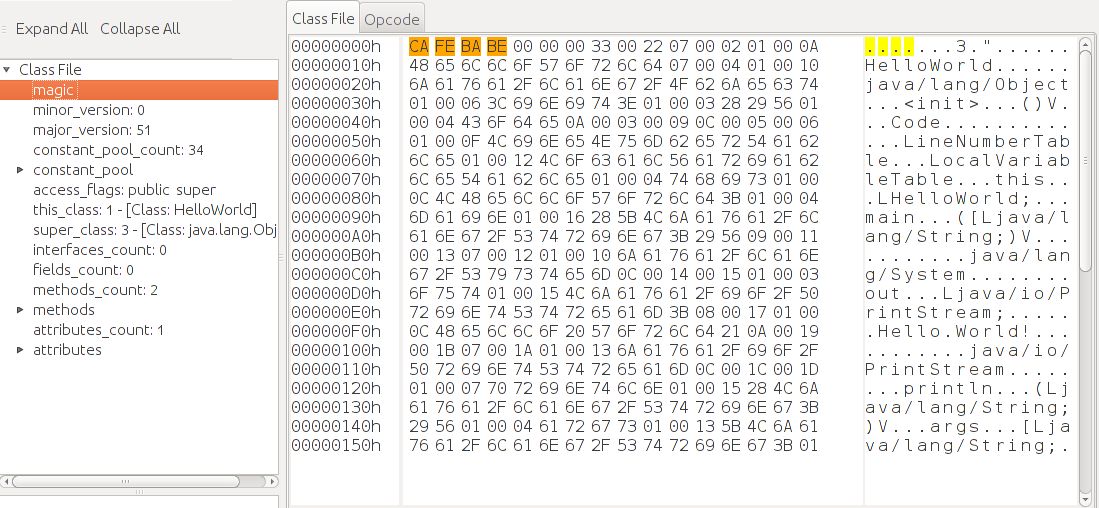
\includegraphics[width=\textwidth]{class1}
\end{center}
\end{frame}

\begin{frame}[fragile]{Classfile Beispiel II}
\begin{center}
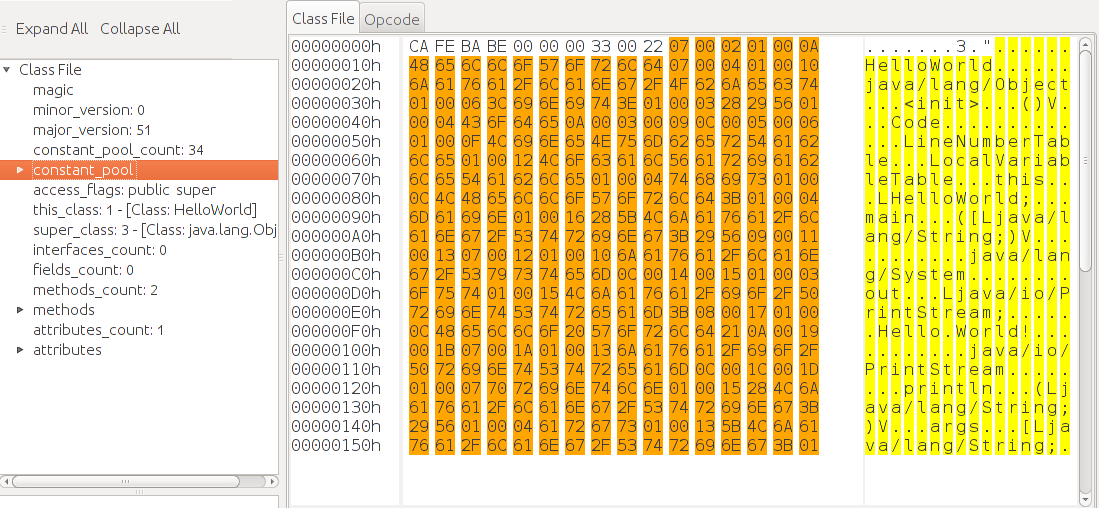
\includegraphics[width=\textwidth]{class2}
\end{center}
\end{frame}

\begin{frame}[fragile]{Classfile Beispiel III}
\begin{center}
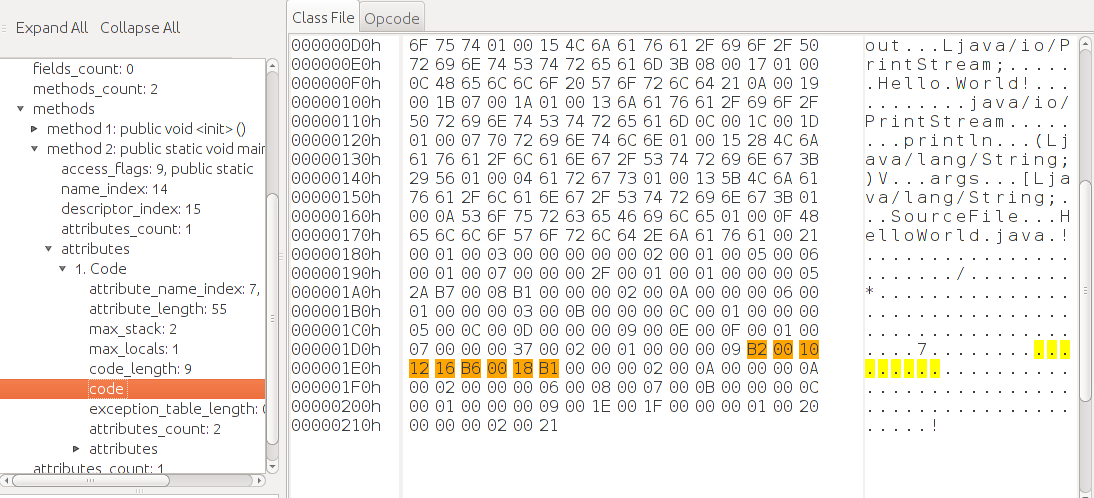
\includegraphics[width=\textwidth]{class3}
\end{center}
\end{frame}

\begin{frame}[fragile]{Classfile Beispiel IV}
\begin{center}
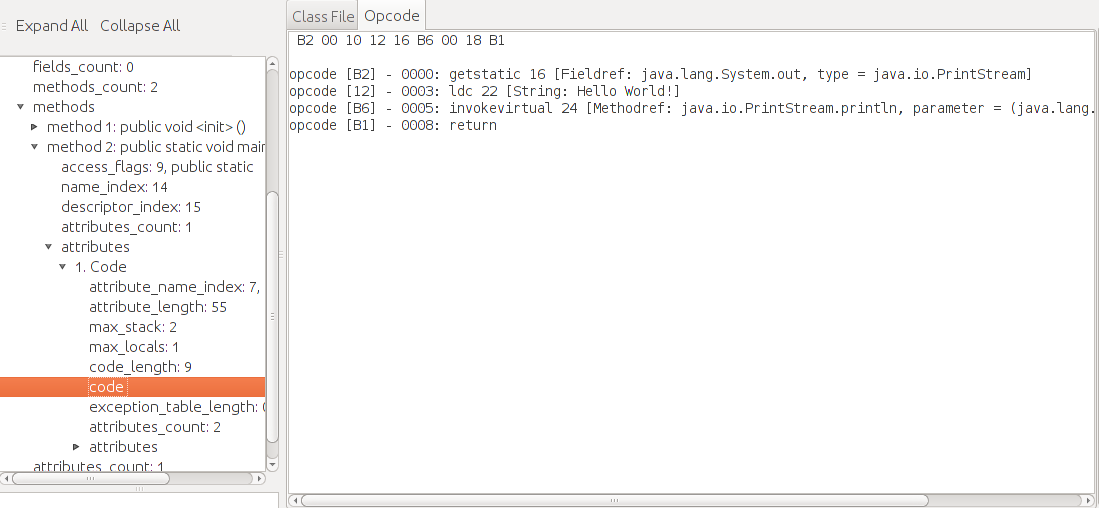
\includegraphics[width=\textwidth]{class4}
\end{center}
\end{frame}

\begin{frame}[fragile]{Backend Klassendiagramm Übersicht}
\begin{center}
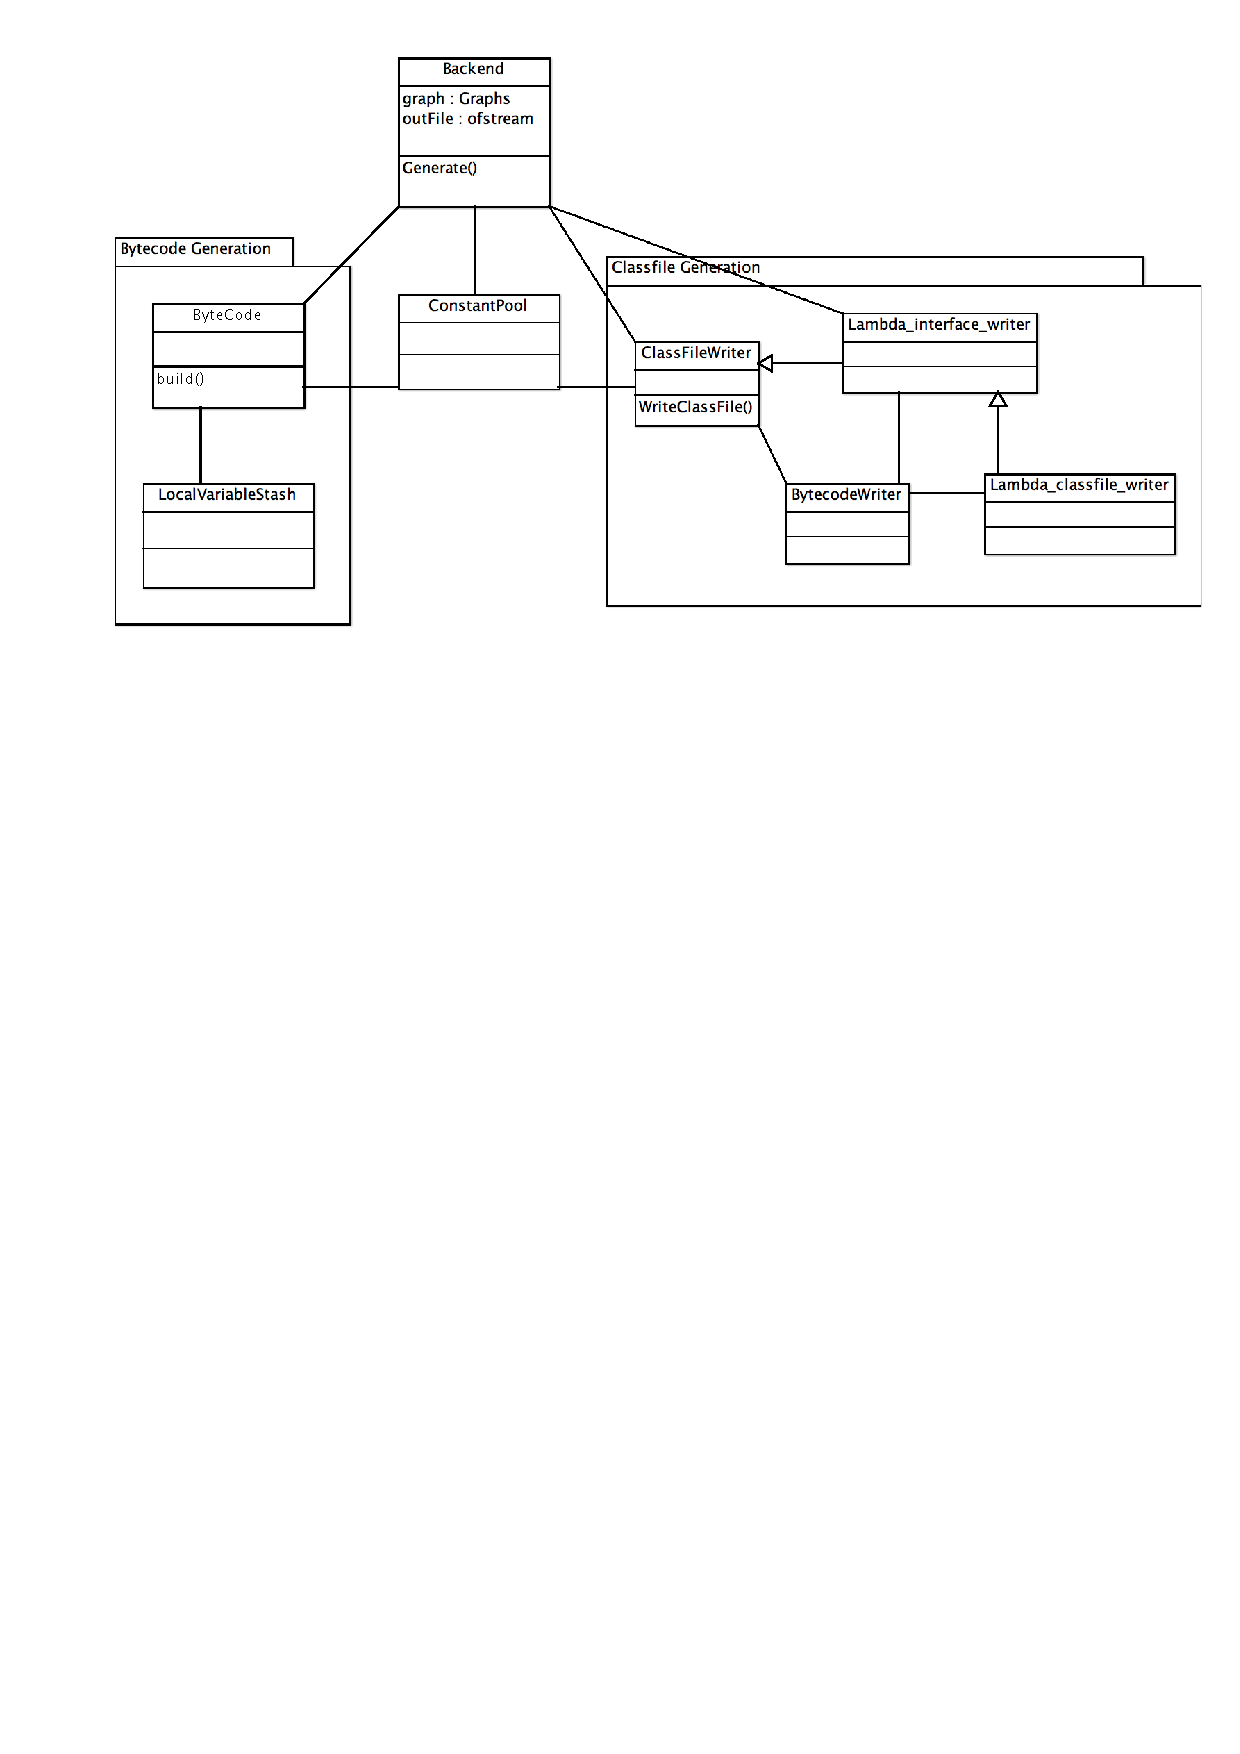
\includegraphics[width=\textwidth]{class}
\end{center}
\end{frame}

\begin{frame}[fragile]{Backend Sequenzdiagramm Übersicht}
\begin{figure}[htp]
\begin{center}
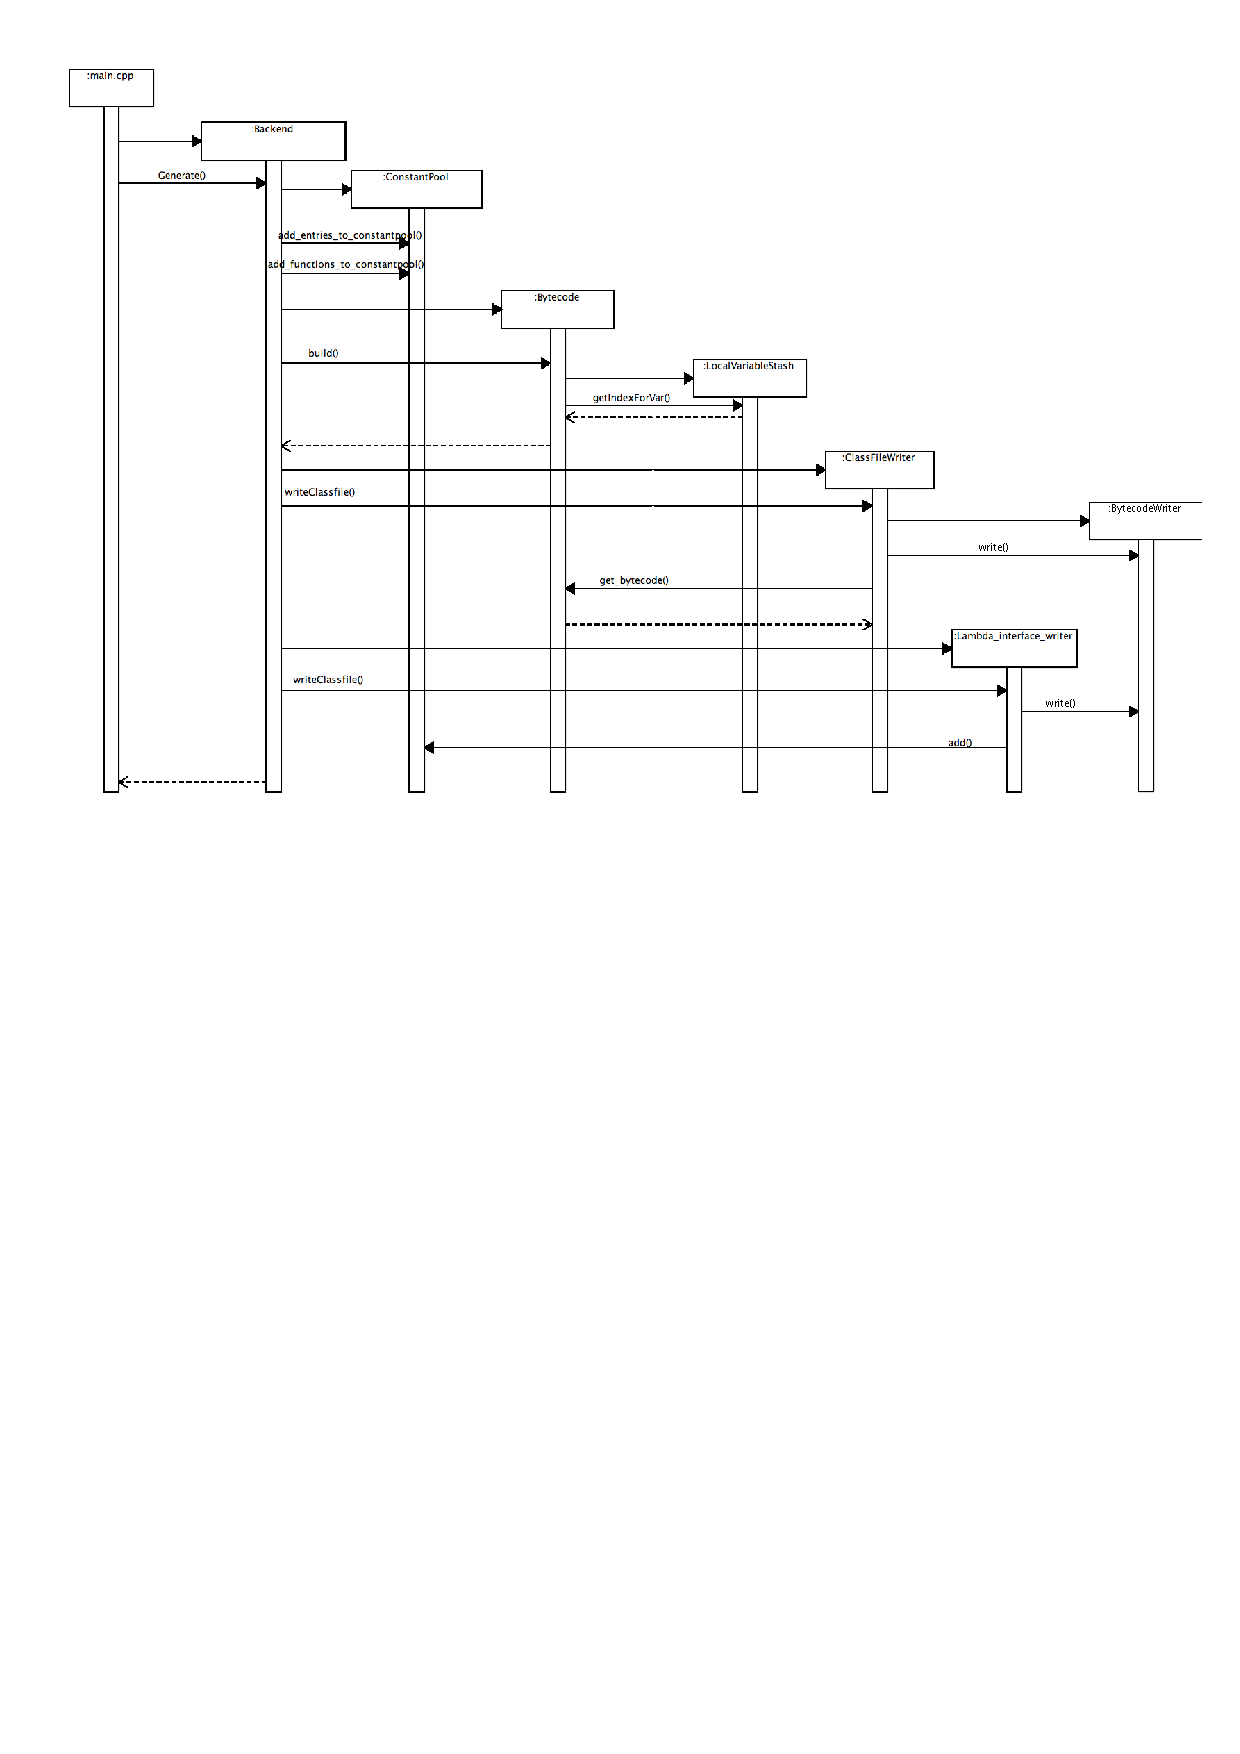
\includegraphics[width=\textwidth]{Sequenz}
\end{center}
\end{figure}
\end{frame}

\begin{frame}[fragile]{Backend Sequenzdiagramm Erster Teil}
\begin{figure}[htp]
\begin{center}
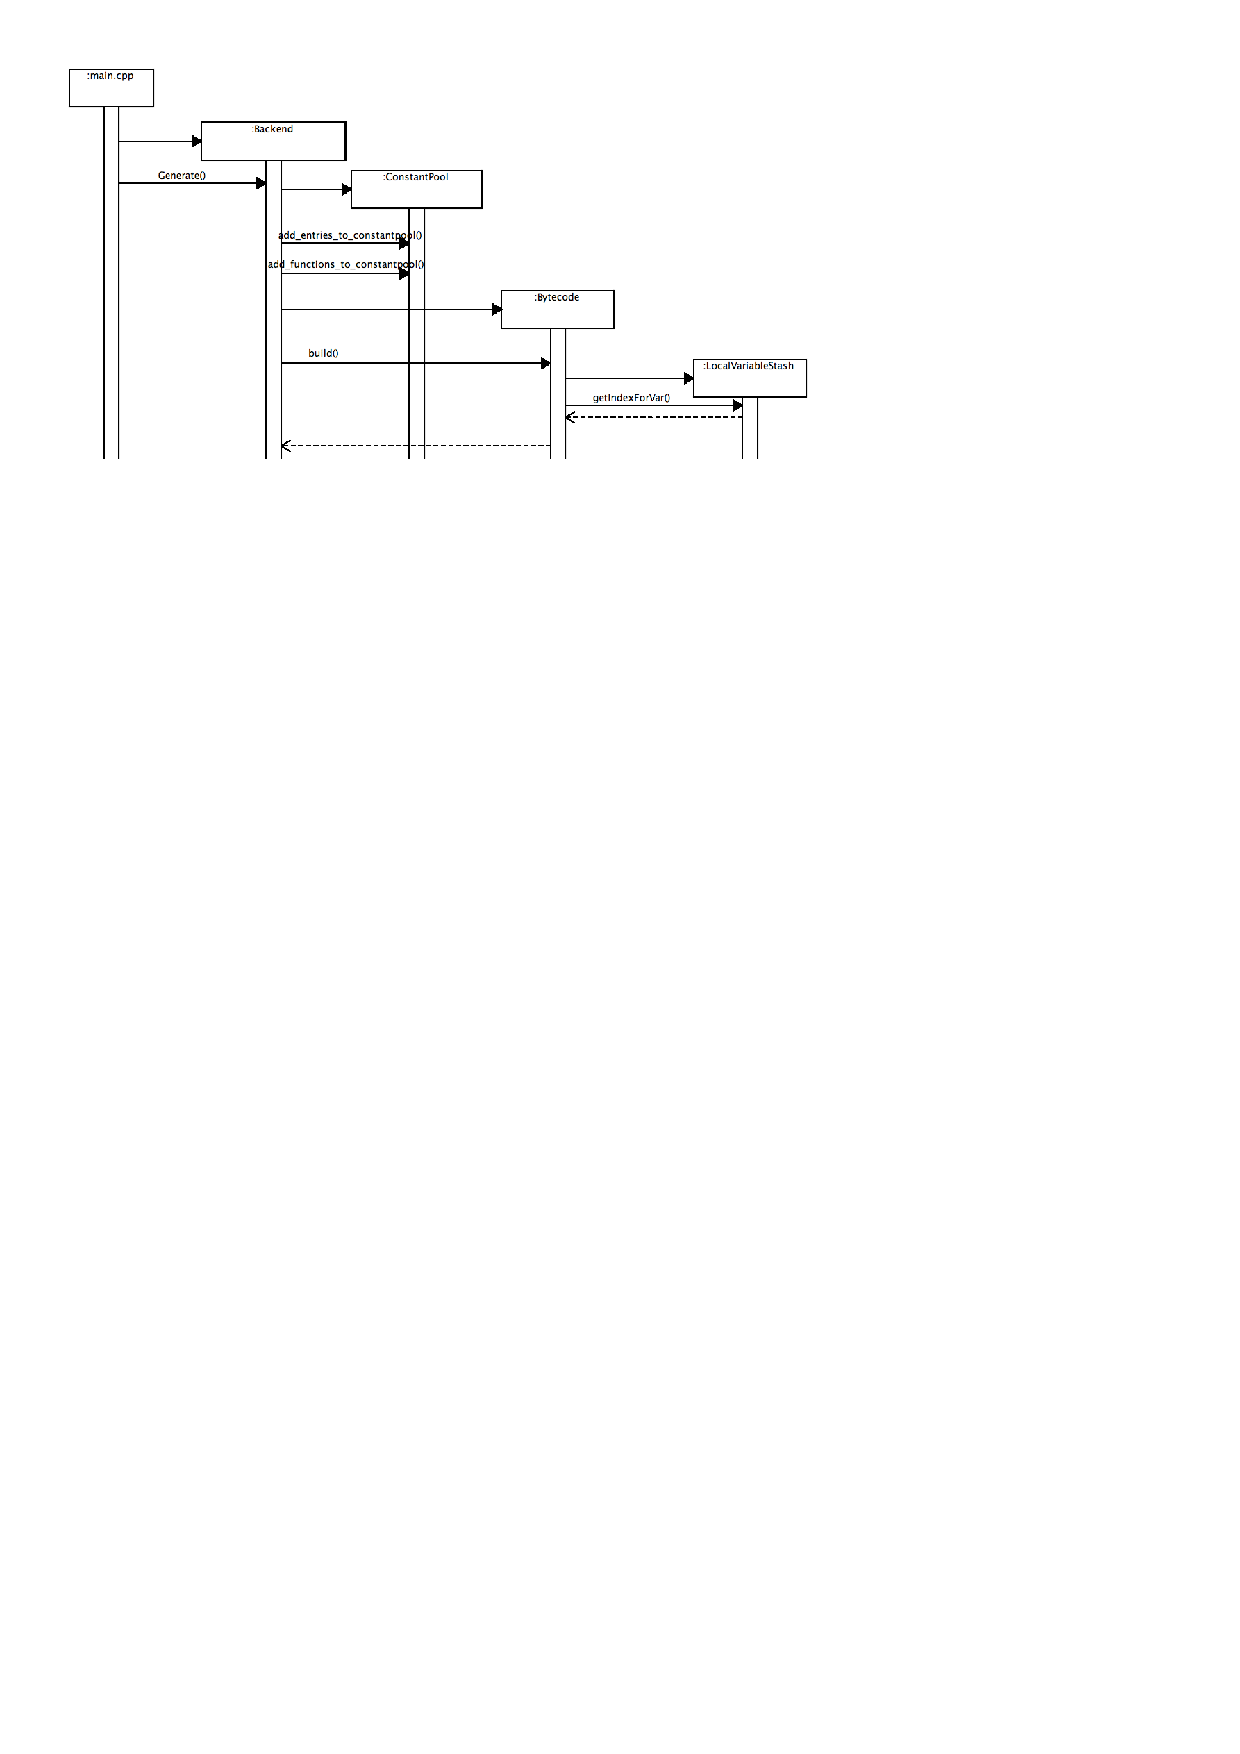
\includegraphics[width=\textwidth]{oben}
\end{center}
\end{figure}
\end{frame}

\begin{frame}[fragile]{Backend Sequenzdiagramm Übersicht}
\begin{figure}[htp]
\begin{center}
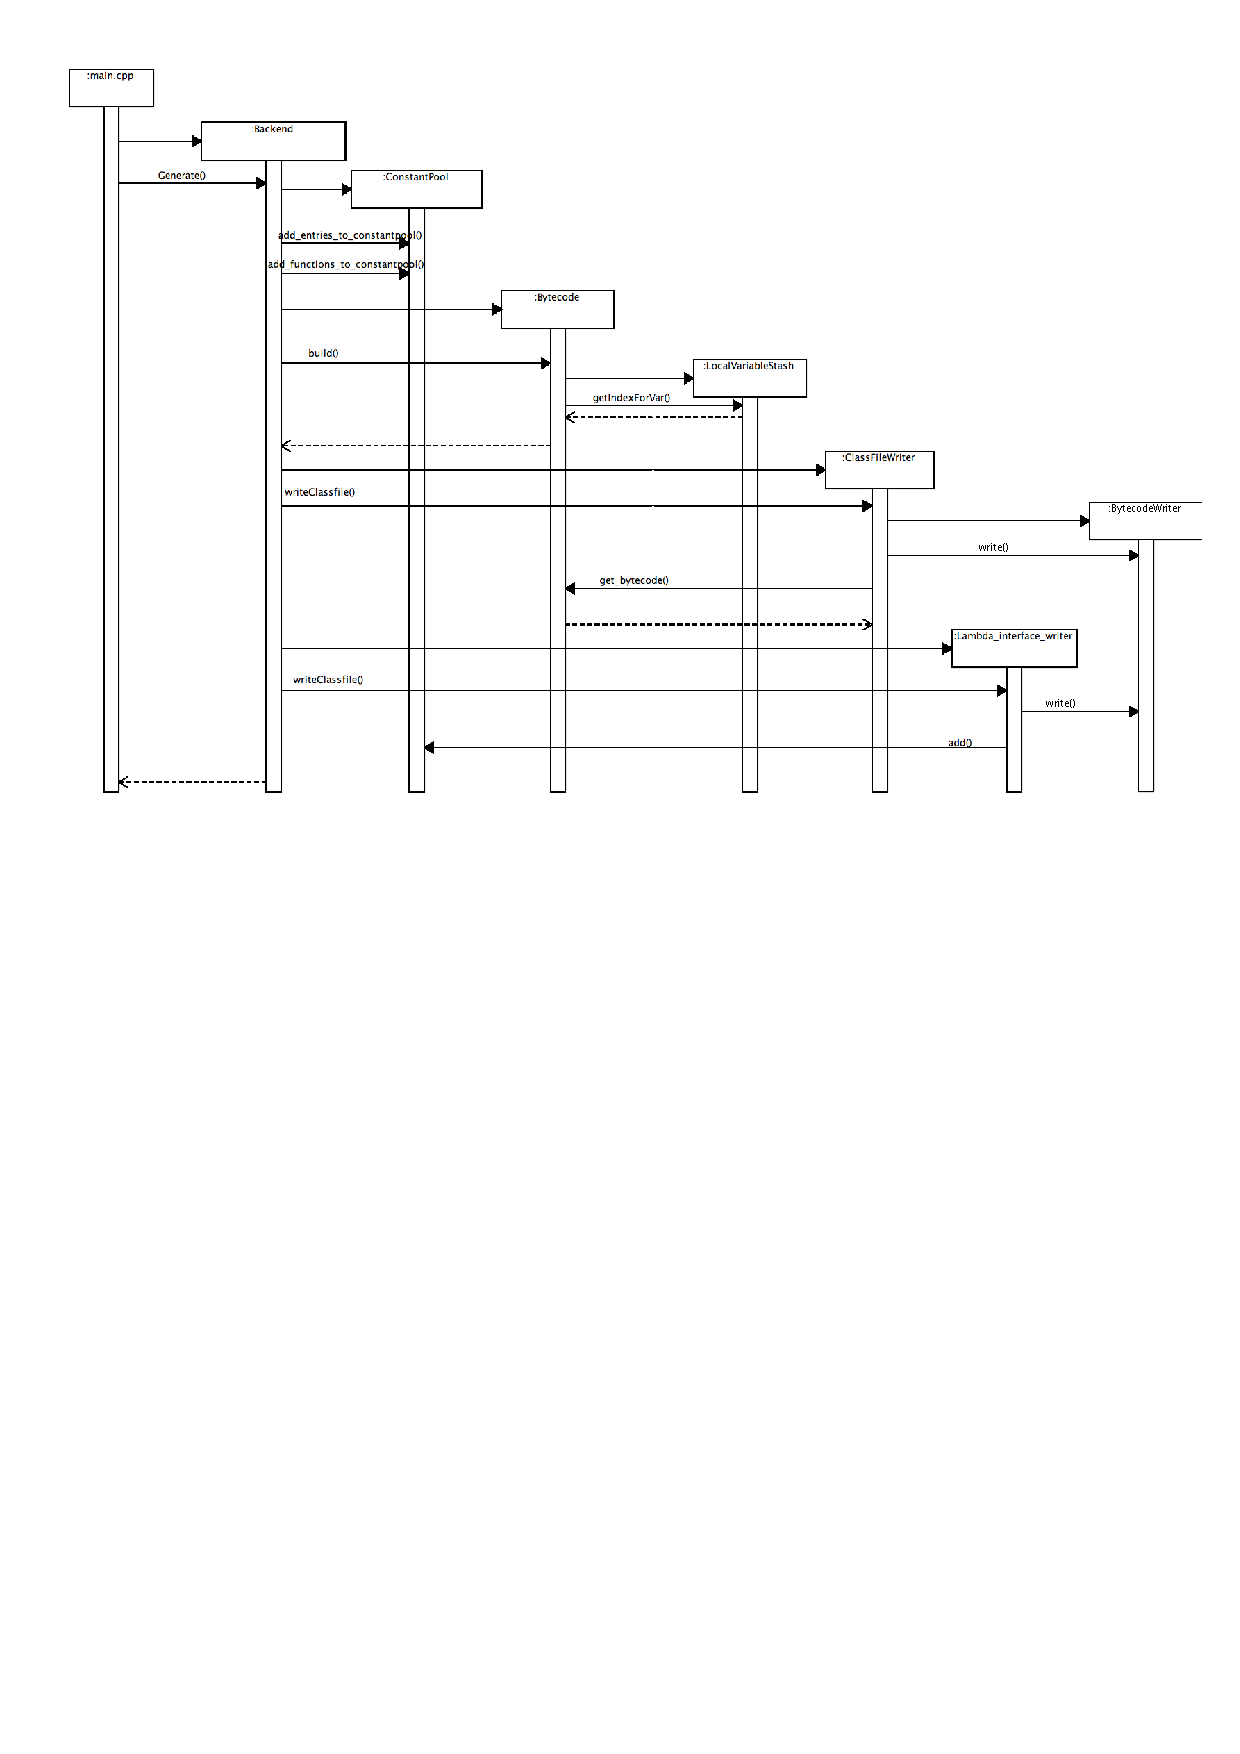
\includegraphics[width=\textwidth]{Sequenz}
\end{center}
\end{figure}
\end{frame}

\begin{frame}[fragile]{Backend Sequenzdiagramm Zweiter Teil}
\begin{figure}[htp]
\begin{center}
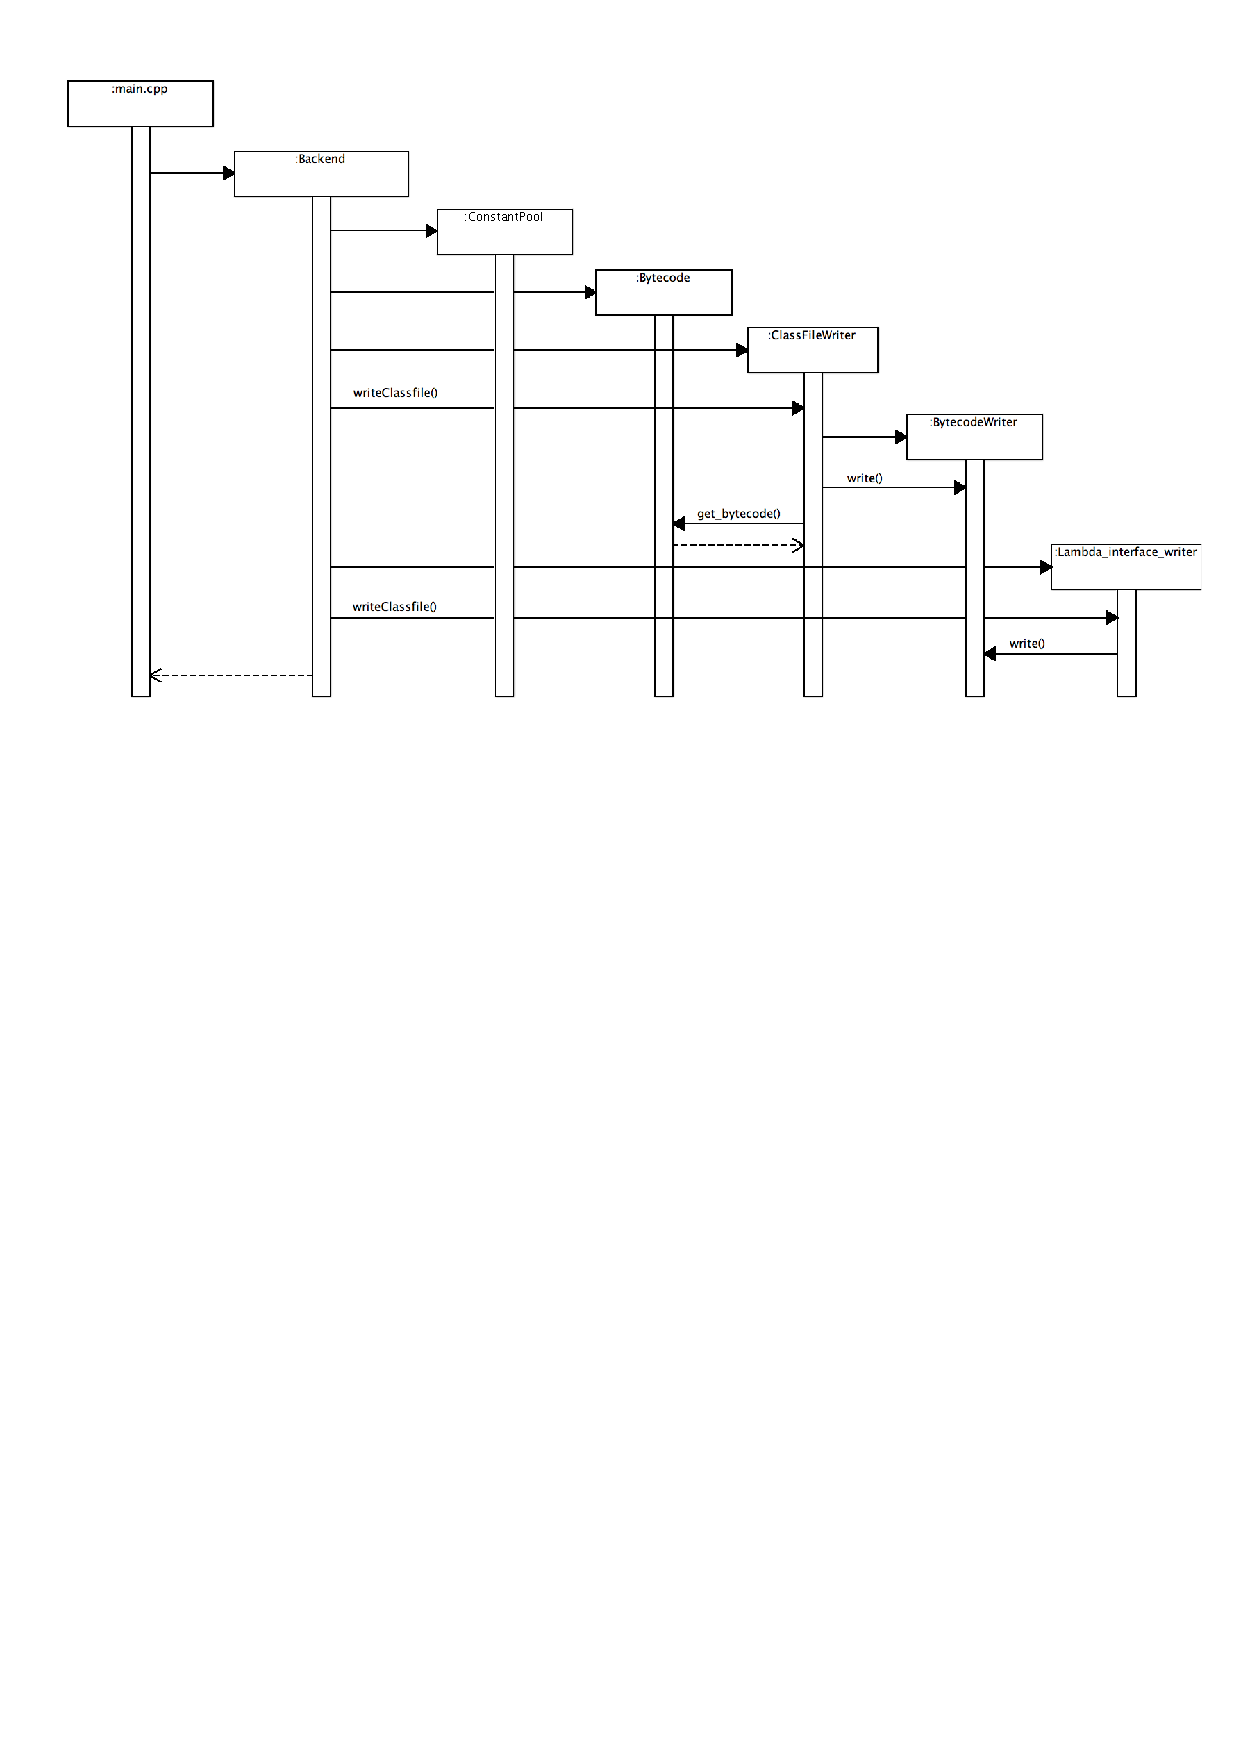
\includegraphics[width=\textwidth]{unten}
\end{center}
\end{figure}
\end{frame}


\begin{frame}[fragile]{Organisation und Probleme}

\pause
Organisation
\pause
  \begin{itemize}
  \item hauptsächlich Teamspeak und Git Kommentarbereich
  \pause
  \item Außerdem XMPP und E-Mail 
  \pause
  \end{itemize}
Probleme
\pause
  \begin{itemize}
  \item Classfiles waren anfangs kompliziert zu durchblicken
  \pause
  \item Das Classfile-Gerüst war schwerer zu realisieren als die grundlegenden Funktionen
  \pause
  \item Einteilung der Milestones war für uns kontraproduktiv
  \end{itemize}
\end{frame}

\begin{frame}[fragile]{Lambda Beispiel: Rail Programm }
Zum Abschluss:
\begin{figure}[htp]
\begin{center}
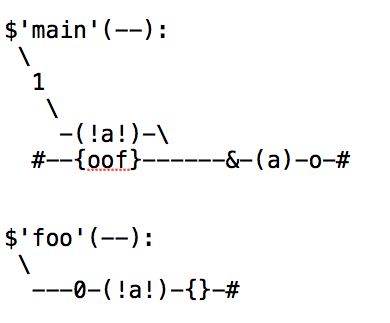
\includegraphics[scale=0.5]{lambda_example}
\end{center}
\end{figure}
\end{frame}

\begin{frame}[fragile]{Lambda Beispiel: Main }
\begin{figure}[htp]
\begin{center}
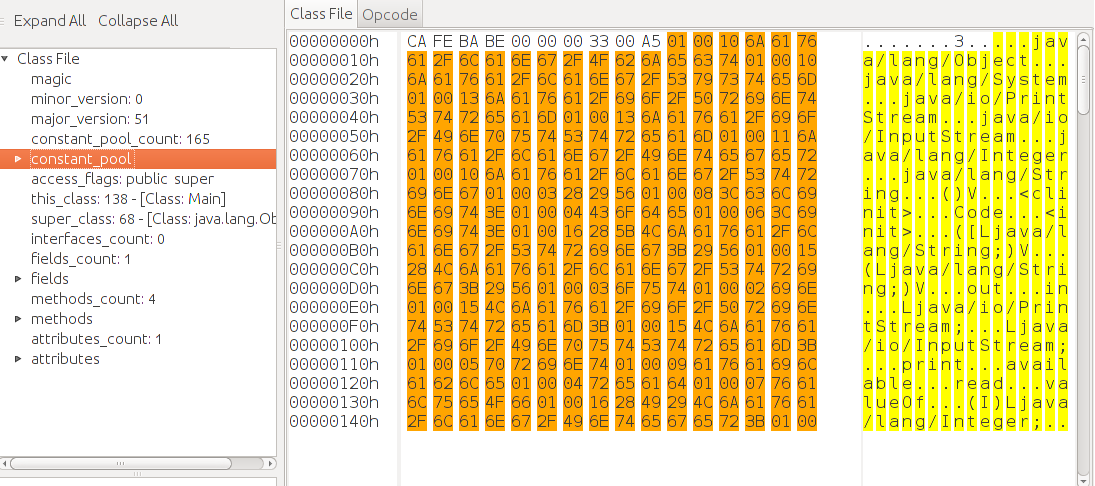
\includegraphics[width=\textwidth]{lambda1}
\end{center}
\end{figure}
\end{frame}

\begin{frame}[fragile]{Lambda Beispiel: Main main }
\begin{figure}[htp]
\begin{center}
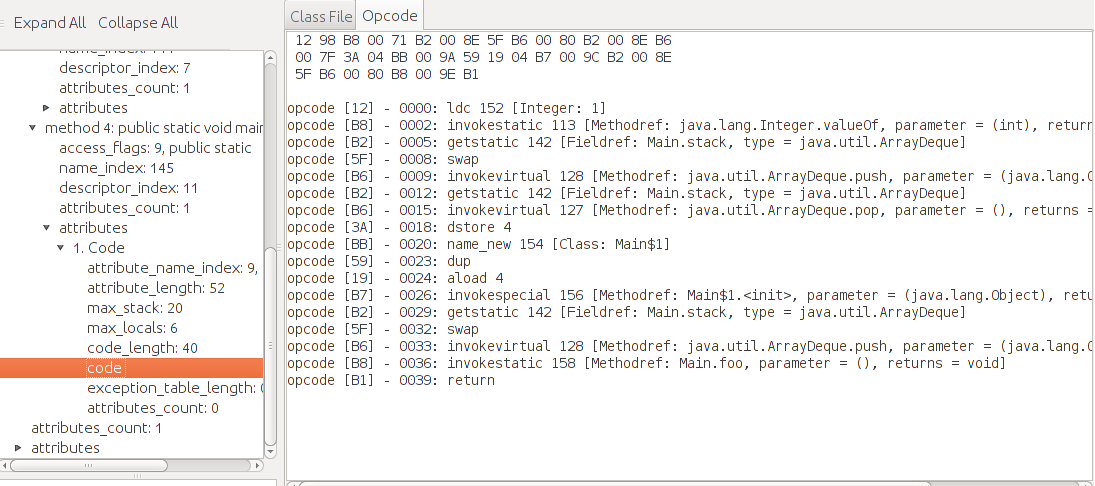
\includegraphics[width=\textwidth]{lambda2}
\end{center}
\end{figure}
\end{frame}

\begin{frame}[fragile]{Lambda Beispiel: Main foo }
\begin{figure}[htp]
\begin{center}
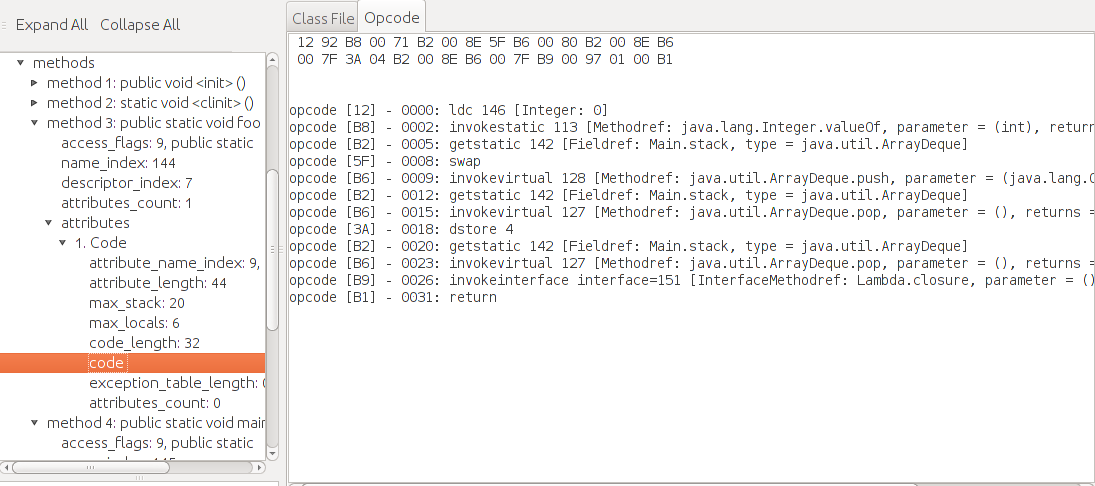
\includegraphics[width=\textwidth]{lambda3}
\end{center}
\end{figure}
\end{frame}

\begin{frame}[fragile]{Lambda Beispiel: Main\$1 closure}
\begin{figure}[htp]
\begin{center}
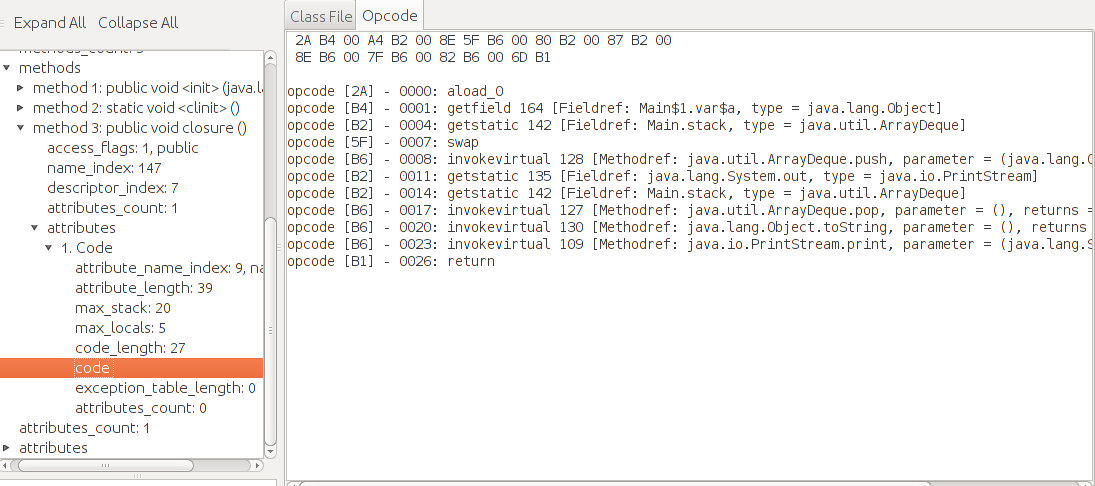
\includegraphics[width=\textwidth]{lambda4}
\end{center}
\end{figure}
\end{frame}